\documentclass[12pt]{report}
\usepackage{amsmath}
\usepackage{amssymb}
\usepackage{graphicx}
\usepackage{hyperref}
\usepackage{color}
\usepackage{float}
\begin{document}	
\title{Relationship between histone sliding and the UV dose}
\maketitle

We set the total length of the chromatin in the initial damage region to be $l$, the number of histones in the damage region embedded in $l$ is $N(t)$, the average number of histones per unit chromatin length is thus $N(t)/l$, we set $\bar{D}$ to be the average number of damage points per unit chromatin length, and set $R(t)$ to be the expansion factor for the radius of the damage region, assuming radially symmetric expansion, with $t$ the time. 

\textbf{Assumptions:} 
\begin{enumerate}
	\item The rate of histones leaving the damage region by sliding is proportional to the damages per nucleosome (linker +histone wrapped DNA);
	\item the rate of expansion is negatively proportional to the rate of histone leaving the damage region by sliding;
	\item The average number of damage points per unit chromatin length is a monotonically increasing function of the UV dose. 
\end{enumerate}

Assumption 1 can be formulated as 
\begin{equation}
\frac{dN(t)}{dt} = -k_n\frac{\bar{D}N(t)}{l}
\end{equation}
with $k_r$ the rate constant and the minus sign indicating depletion. Using the initial condition $N(0) = N_0$, the solution is given by 
\begin{equation}
N(t) = N_0\exp(-\frac{k_r\bar{D}t}{l})
\end{equation}
We note that even if the linker DNA between histone lengthen, then sliding a histone on the linker DNA wraps on the histone on average the same amount of damages as were before sliding. Therefore it will continue sliding to keep exposing damage sites.

From assumption 2 we can write 
\begin{equation}
\frac{dR(t)}{dt}=-k_R\frac{dN(t)}{dt}
\end{equation}
with the initial condition $R(0)=1$ we find 
\begin{equation}\label{eq:expansionFactor}
R(t) = 1+k_RN_0(1-\exp(-\frac{k_r\bar{D}t}{l}))
\end{equation}

The total number of histone loss is obtained at $t_{15}$ post UVC and is written as  
\begin{equation}
h(t_{15}) = \frac{R(t_{15})-1}{R(t_{15})} +\frac{N_0-N(t_{15})}{N_0R(t_{15})}=1-\frac{N(t_{15})}{N_0R(t_{15})}
\end{equation}
substituting $t=t_{15}$ in the expressions for $N(t)$ and $R(t)$ and plugging into the equation for $h(t_{15})$ we obtain 
\begin{equation}\label{eq:totalHistoneLoss}
h(t_{15})=1-\frac{\exp(-\frac{k_r\bar{D}}{l}t_{15})}{ 1+k_RN_0(1-\exp(-\frac{k_r\bar{D}}{l}t_{15}))}
\end{equation}

The expression on the right-hand side of \ref{eq:totalHistoneLoss} can now be regarded as function of the average number of damage points per unit length, $\bar{D}$. Using assumption 3 above, $\bar{D}$ increases with the UV dose at least linearly and decreases with the distance from focal point. The decrease of UVC intensity, $I$,  with distance from the its focal point is assumed to follow the inverse-square law of laser intensity. That is, $I\propto U/r^2$, with $r$ the distance from focal point. 

Assuming a uniform distribution of DNA, the amount of DNA enclosed in concentric rings around the focal point increases linearly with $r$. Therefore, the expected number of damages in each concentric ring is $D(r)\propto rU/r^2=U/r$. 
The average of $\bar{D}(R)$ in a circular region of radius $R$ is then proportional to 
\begin{equation}
\bar{D}(R)\propto \int_0^R r/r dr = UR
\end{equation}
and the average number of damages per unit length is thus proportional to $U$.

We therefore substitute this estimation into \ref{eq:totalHistoneLoss} to obtain the total loss of histones as a function of the UV dose at $t_{15}$
\begin{equation}\label{eq:totalHiostoneLossVsUV}
h(t_{15})=1-\frac{\exp(-\frac{k_rt_{15}}{l}U)}{ 1+k_RN_0(1-\exp(-\frac{k_rt_{15}}{l}U))}
\end{equation}
 
By fitting to the data a model of the type \ref{eq:totalHiostoneLossVsUV} we obtain 
\begin{figure}[H]
\centering
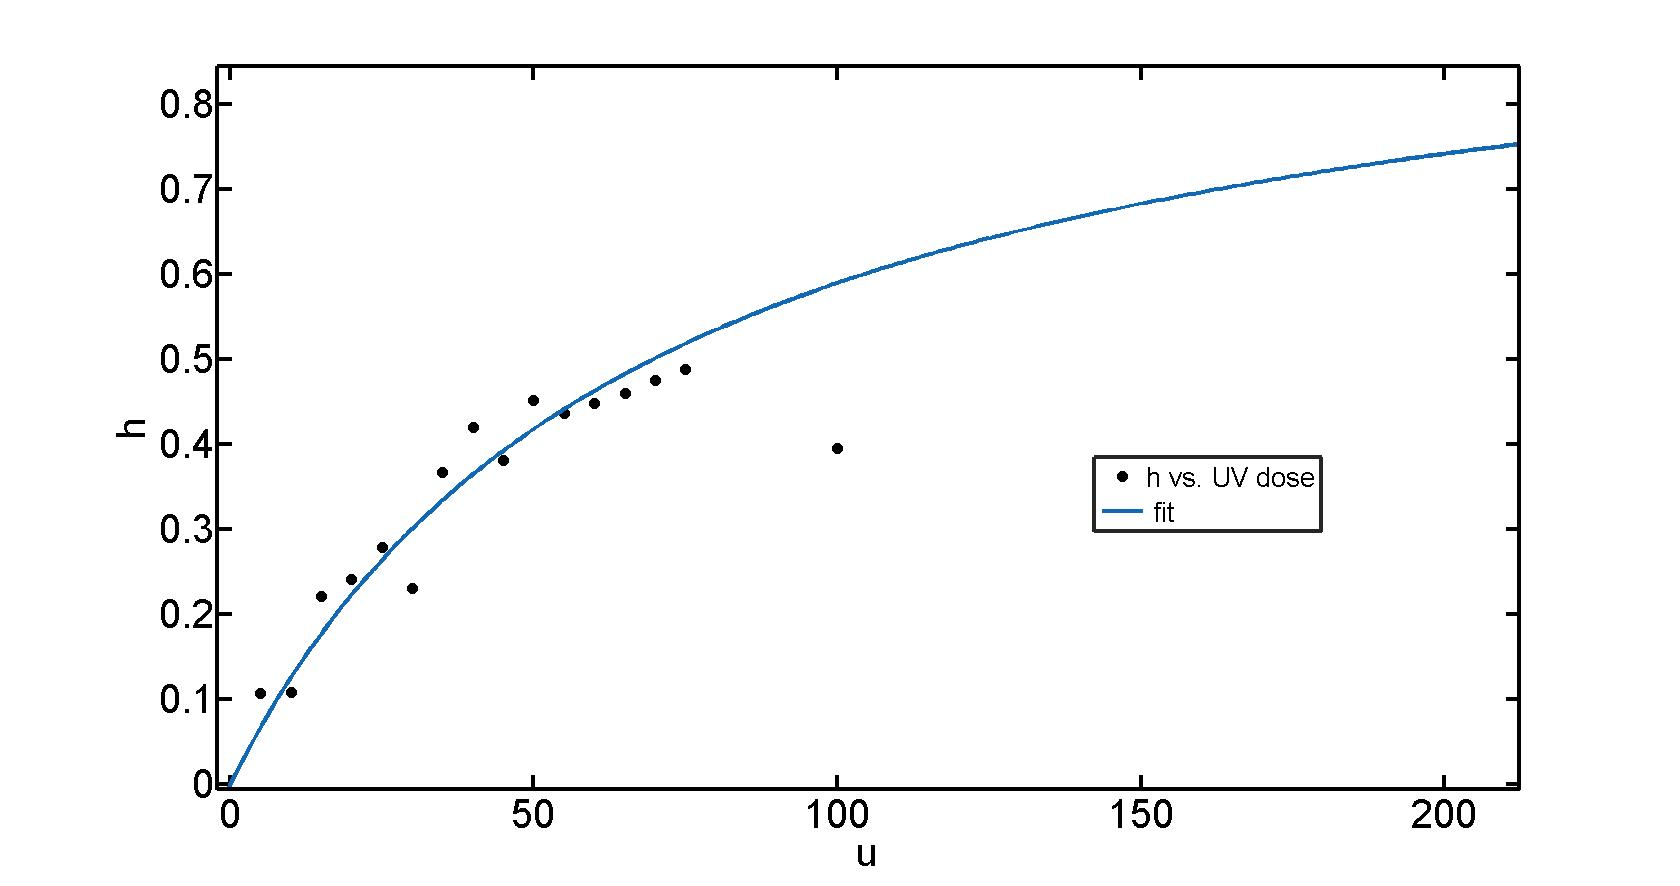
\includegraphics[width=0.5\linewidth, height=0.3\textheight]{images/hVsUVDoseModelFit01}
\caption{Fitting of the model in \ref{eq:totalHiostoneLossVsUV} to the experimental data}
\label{fig:hVsUVDoseModelFit01}
\end{figure}

The DNA loss at $t_{15}$ is a function of the expansion factor $R(t)$ and is given by 
\begin{equation}\label{eq:dStSt}
d= 1-1/R 
\end{equation}
substituting the expression for $R$ from \ref{eq:expansionFactor} into \ref{eq:dStSt}, we obtain 
\begin{equation}
d =  \frac{k_RN_0(1-\exp(-\frac{k_rt_{15}}{l}U))}{(1+k_RN_0(1-\exp(-\frac{k_rt_{15}}{l}U)))}
\end{equation}

From the fitting for $h$ we have $k_rt_{15}/l = 2\time10^-5 \quad k_RN_0 = 747$. Plugging these values and examining the resulted plot vs the experimental data for $d$ we have 


\end{document}

